\documentclass{article}
\usepackage[utf8]{inputenc}
\usepackage{amsmath}
\usepackage{graphicx}
\usepackage{placeins}
\usepackage{subfig}
\usepackage{adjustbox}
\usepackage[table,xcdraw]{xcolor}

\title{MTRN4030 Exercise 2}
\author{Zachary Hamid}
\date{October 2019}

\begin{document}

\maketitle
\section{Part 1 - Line Search and Gradient-based Optimization}
\subsection{Task 1}
\paragraph*{1.} Assuming we start with some search range $[a_{0},b_{0}]$ and a unimodal objective function, $f$, we choose two new points, $a_{1}$ and $b_{1}$ to evaluate the function $f$ at in order to determine where the minimum (or maximum) is located. These points are chosen such that the reduction in range is symmetric, therefore:
\begin{equation}
    a_{1} - a_{0} = b_{1} - b_{0} = \rho(b_{0}-a_{0}), \rho < 0.5
\end{equation}
\begin{figure}[!h]
    \centering
    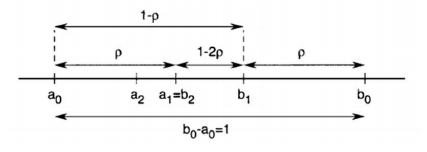
\includegraphics[scale=0.8]{task1/task1-2.png}
    \caption{Finding value of $\rho$ resulting in only one new evaluation of $f$ [CITATION NEEDED]}
    \label{fig:task1-1}
\end{figure}
So for only one new evaluation of $f$, we choose $\rho$ such that:
\begin{equation*}
    \rho(b_{1} - a_{0}) = b_{1} - b_{2}
\end{equation*}
Since $b_{1} - a_{0} = 1 - \rho$, and $b_{1} - b_{2} = 1 - 2\rho$:
\begin{equation*}
    \rho(1 - \rho) = 1 - 2\rho
\end{equation*}
We then get a quadratic equation from which we can solve for $\rho$:
\begin{eqnarray*}
    \rho^{2} - 3\rho + 1 = 0
\end{eqnarray*}
Since it is required that $\rho < 0.5$ the solution that is taken from this quadratic is:
\begin{equation*}
    \rho = (3 −\sqrt{5})/2 \approx 0.382.
\end{equation*}

\paragraph*{2.} Given an objective function $f(\mathbf{x})$ with the assumption that the functions is continuous where derivatives exist, the Taylor series expansion about a point $\mathbf{x}_{n}$ up to the quadratic term can be given as:
\begin{equation*}
    f(\mathbf{x}) \approx f(\mathbf{x}_{n}) + (\mathbf{x} - \mathbf{x}_{n})\nabla f(\mathbf{x}_{n}) + \frac{1}{2}(\mathbf{x} - \mathbf{x}_{n})^{T}\nabla^{2}f(\mathbf{x}_{n})(\mathbf{x} - \mathbf{x}_{n})
\end{equation*}
Where $\nabla f(\mathbf{x}_{n})$ is the gradient of the function $f(\mathbf{x})$ at the point $\mathbf{x}_{n}$, and $\nabla^{2} f(\mathbf{x}_{n})$ is the Hessian matrix of the function $f(\mathbf{x})$ at the point $\mathbf{x}_{n}$.



\paragraph*{3.}
From the Taylor series expansion given above setting $\Delta \mathbf{x} = \mathbf{x} - \mathbf{x}_{n}$ we have:
\begin{equation}
    f(\mathbf{x}) \approx f(\mathbf{x}_{n}) + \Delta \mathbf{x}\nabla f(\mathbf{x}_{n}) + \frac{1}{2}\Delta \mathbf{x}^{T}\nabla^{2}f(\mathbf{x}_{n})\Delta \mathbf{x}
\end{equation}
From this, the derivative with respect to the infinitesimal change $\Delta \mathbf{x} = \mathbf{x} - \mathbf{x}_{n}$ can be found to be:
\begin{align*}
    \frac{df(\mathbf{x})}{d\Delta \mathbf{x}} &= \nabla f(\mathbf{x}_{n}) + 0.5\frac{d(\Delta \mathbf{x}^{T}\nabla^{2}f(\mathbf{x}_{n})\Delta \mathbf{x})}{d\Delta \mathbf{x}}\\
    &= \nabla f(\mathbf{x}_{n}) + 0.5(2\nabla^{2}f(\mathbf{x}_{n})\Delta \mathbf{x})\\
    &= \nabla f(\mathbf{x}_{n}) + \nabla^{2}f(\mathbf{x}_{n})\Delta \mathbf{x}
\end{align*}



\paragraph*{4.}
Applying the first order necessary condition (FONC) to the derivative of the Taylor series expansion of objective function $f(\mathbf{x})$, given in 3. above:
\begin{equation}
    \frac{df(\mathbf{x})}{d\Delta \mathbf{x}} = \mathbf{0} = \nabla f(\mathbf{x}_{n}) + \nabla^{2}f(\mathbf{x}_{n})\Delta \mathbf{x}
\end{equation}
Rearranging for $\mathbf{x}$, we get an iterative formula that finds the optimal value for $\mathbf{x}$ (ie. $\mathbf{x}^{*}$):
\begin{equation}
    \mathbf{x}_{n+1} = \mathbf{x}_{n} - (\nabla^{2}f(\mathbf{x}_{n}))^{-1}\nabla f(\mathbf{x}_{n})
\end{equation}
The iterative formula above is known as Newton's Method.



\paragraph*{5.}


\subsection{Task 2}
The solution derived by the 2-dimensional Golden Ratio search method using Matlab is shown in the figures below:
\FloatBarrier
\begin{figure}[h!]
\begin{adjustbox}{max width=1.5\linewidth,center}
    \centering
    \subfloat[x-y view of solution]{{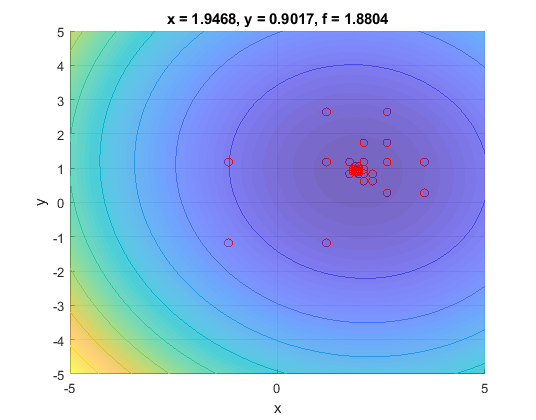
\includegraphics[width=10cm]{task2/task2-1.png} }}%
    \subfloat[3D view of function]{{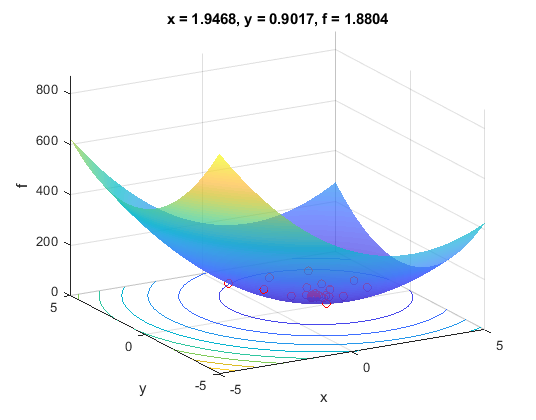
\includegraphics[width=10cm]{task2/task2-2.png} }}%
\end{adjustbox}
    \caption{Solution to task 2 using 2-dimensional Golden Ratio search algorithm}
    \label{fig:task2}%
\end{figure}
\FloatBarrier
\noindent This solution can be verified by inspection of the characteristics of both the gradient vector and Hessian matrix of the function:
\begin{equation*}
    f(x,y) = 10(x-2)^{2} + xy + 10(y-1)^{2}
\end{equation*}
The gradient vector was found to be:
\begin{equation*}
    \nabla f = \begin{bmatrix}\delta f / \delta x \\ \delta f / \delta y\end{bmatrix} = \begin{bmatrix} 20x + y - 40\\ x + 20y - 20\end{bmatrix}
\end{equation*}
To locate the optimum design variables $x^{*}$, $y^{*}$, the first-order condition of $\nabla f = 0$ must be satisfied.
\begin{eqnarray}\label{eq:rearrange-1}
    \frac{\delta f}{\delta x} = 20x + y - 40 = 0 \\\label{eq:subst-1}
    \frac{\delta f}{\delta y} = x + 20y - 20 = 0
\end{eqnarray}
Rearranging Eq. \ref{eq:rearrange-1} gives:
\begin{equation}\label{eq:rearrange-2}
    y = 40 - 20x
\end{equation}
Substituting Eq. \ref{eq:rearrange-2} into Eq. \ref{eq:subst-1} and solving for $x$ gives:
\begin{equation*}
    x = \frac{780}{399} \approx 1.95489
\end{equation*}
Substituting the above result into Eq. \ref{eq:rearrange-2} gives:
\begin{equation*}
    y = \frac{120}{133} \approx 0.90226
\end{equation*}
Therefore an optimum $(x^{*}, y^{*})$ occurs at $(1.95489, 0.90226)$. To determine if this is a minimum (as required by the task description), the Hessian matrix characteristics must be inspected. The Hessian matrix can be defined as:
\begin{equation*}
    H = \nabla^{2}f = \begin{bmatrix} 
\delta f / \delta x^{2} & \delta f / \delta x \delta y \\
\delta f / \delta y \delta x & \delta f / \delta y^{2}
\end{bmatrix} = \begin{bmatrix}20 & 1 \\ 1 & 20\end{bmatrix}
\end{equation*}
The condition for the optimum point $(x^{*}, y^{*})$ to be a minimum is the Hessian matrix must be positive definite, that is, $\nabla^{2} f > 0$. The method of principal minors can be used to determine this. This method looks at the determinants of the leading principal submatrices of the Hessian matrix. If these are all positive, the Hessian is positive definite.
\begin{equation*}
    A_{0} = \begin{vmatrix} 20 \end{vmatrix} = 20 > 0\\
\end{equation*}
\begin{equation*}
    A_{1} =\begin{vmatrix} 20 & 1 \\ 1 & 20 \end{vmatrix} = 20*20 - 1*1 = 400 - 1 = 399 > 0
\end{equation*}
Since both $A_{0}$ and $A_{1}$ are positive, the Hessian matrix H is positive definite and therefore the optimum $(x^{*}, y^{*})$ found above is a minimum. Substituting this optimal value into the original function gives the minimum function value:
\begin{equation*}
    f(1.95489, 0.90226) \approx 1.8797
\end{equation*}
It can be seen that these values of $x^{*}, y^{*}$ and $f$ are all very similar to what was found using the Golden Section search method.



%%%%%%%%%%%%%%%%% TASK 3 %%%%%%%%%%%%%%%%%%%%%%%%%%
\subsection{Task 3}
Applying Newton's Method to the function given in question 6 of this task resulted in the minimum being found within a single iteration. To determine why this is the case, the objective function is first expanded:
\begin{equation*}
    f(x,y) = (x-1)^{2} + (y-2)^{2} = x^{2} + y^{2} - 2x - 4y + 5
\end{equation*}
This function can then be reformulated as:
\begin{equation} \label{eq:task3}
    f(x,y) = \frac{1}{2}\mathbf{x}^{T}\mathbf{Qx}-\mathbf{x}^{T}\mathbf{b} + c
\end{equation}
Where:
\begin{equation*}
    \mathbf{Q} = \begin{bmatrix} 2 & 0 \\ 0 & 2 \end{bmatrix}, \mathbf{b} = \begin{bmatrix} 2 \\ 4\end{bmatrix}, \mathbf{x} = \begin{bmatrix} x \\ y \end{bmatrix}, c = 5
\end{equation*}
In order for Newton's Method to converge from any initial point to the optimum in a single iteration, a few criteria must be met. Firstly, it is required that the gradient vector, $\mathbf{g} = \nabla f(x,y) = \mathbf{Qx} - \mathbf{b}$:
\begin{equation*}
    \nabla f(x,y) = \begin{bmatrix} 2x - 2 \\ 2y - 4\end{bmatrix} = \begin{bmatrix} 2 & 0 \\ 0 & 2\end{bmatrix}\begin{bmatrix}x \\ y\end{bmatrix} - \begin{bmatrix} 2 \\ 4 \end{bmatrix}= \mathbf{Qx} - \mathbf{b}
\end{equation*}
\noindent Additionally, the Hessian matrix, $\mathbf{H}$ must be equal to $\mathbf{Q}$:
\begin{equation*}
    \mathbf{H} = \nabla^{2}f(x,y) = \begin{bmatrix} 2 & 0 \\ 0 & 2 \end{bmatrix} = \mathbf{Q}
\end{equation*}
\noindent Finally, $\mathbf{Q}$ needs to be symmetric and invertible:
% Q' = Q
\begin{equation*}
    \mathbf{Q}^{T} = \begin{bmatrix} 2 & 0 \\ 0 & 2 \end{bmatrix}^{T} = \begin{bmatrix} 2 & 0 \\ 0 & 2 \end{bmatrix} = \mathbf{Q}
\end{equation*}
\begin{equation*}
    \mathbf{Q^{-1}} = \frac{1}{4}\begin{bmatrix} 2 & 0 \\ 0 & 2 \end{bmatrix} = \begin{bmatrix} 0.5 & 0 \\ 0 & 0.5 \end{bmatrix}
\end{equation*}
Now, from Newton's Method we have:
\begin{equation*}
    \mathbf{x}^{k+1} = \mathbf{x}^{k} - \mathbf{H(x}^{k})^{-1}\mathbf{g}^{k}
\end{equation*}
Substituting the results of $\mathbf{H} = \mathbf{Q}$ and $\mathbf{g} = \mathbf{Qx} - \mathbf{b}$ in and setting k = 0 since it is the first iteration:
\begin{align*}
    \mathbf{x}^{1} &= \mathbf{x}^{0} - \mathbf{H(x}^{0})^{-1}\mathbf{g}^{0}\\
    &= \mathbf{x}^{0} - \mathbf{Q}^{-1}[\mathbf{Qx}^{0} - \mathbf{b}] = \mathbf{Q}^{-1}\mathbf{b}
\end{align*}
The optimal point $\mathbf{x}^{*}$ occurs when $\mathbf{g} = \nabla f(x,y) = \mathbf{0}$, therefore:
\begin{align*}
    \mathbf{Qx} - \mathbf{b} &= \mathbf{0}\\
    \mathbf{Qx} &= \mathbf{b}\\
    \mathbf{x} &= \mathbf{Q}^{-1}\mathbf{b} = \mathbf{x}^{*}
\end{align*}

\noindent So it can be seen that, on iteration 1 (ie. when calculating $\mathbf{x}^{1}$) the result is the optimum $\mathbf{x}^{*}$, regardless of which initial point $\mathbf{x}^{0}$ is used. From this result, the exact point where the minimum occurs can be calculated for the objective function given in Eq. \ref{eq:task3}, and is given below:
\begin{equation*}
    \mathbf{x}^{1} = \mathbf{x}^{*} = \begin{bmatrix} 0.5 & 0 \\ 0 & 0.5 \end{bmatrix} \begin{bmatrix} 2 \\ 4 \end{bmatrix}  = \begin{bmatrix} 1 \\ 2\end{bmatrix}
\end{equation*}
Substituting this result into the original objective function yields the minimum function value:
\begin{equation*}
    f(1,2) = (1-1)^{2} + (2-2)^{2} = 0
\end{equation*}
This result is consistent with the results shown in question 6 of the exercise 2 document.





\section{Part 2 - Mechanical System Design}
\subsection{Task 4}
The bracketing method employed for this task resulted in an initial search range of $\lambda \in [0.31, 0.91]$ for each method. From this, the number of iterations to find the optimal value of $\lambda$ as well as the maximum function value corresponding to this $\lambda$ is shown in the table below:
\FloatBarrier
\begin{table}[h!]
\centering
\begin{tabular}{c|
>{\columncolor[HTML]{EFEFEF}}c |
>{\columncolor[HTML]{EFEFEF}}c |}
\cline{2-3}
\multicolumn{1}{l|}{}                                                                                         & \cellcolor[HTML]{C0C0C0}{\color[HTML]{000000} Fibonacci} & \cellcolor[HTML]{C0C0C0}{\color[HTML]{000000} Bisection} \\ \hline
\multicolumn{1}{|c|}{\cellcolor[HTML]{C0C0C0}\begin{tabular}[c]{@{}c@{}}Number of \\ Iterations\end{tabular}} & 3                                                        & 5                                                        \\ \hline
\multicolumn{1}{|c|}{\cellcolor[HTML]{C0C0C0}\begin{tabular}[c]{@{}c@{}}Maximum \\ Value $f(\lambda)$\end{tabular}}        & 0.3076                                                   & 0.31                                                     \\ \hline
\end{tabular}
\end{table}
\FloatBarrier
\noindent It can be seen that the Fibonacci method obtained the approximate optimal value in fewer iterations.

In terms of implementation complexity, each method has their own drawbacks, with the Fibonacci Method having computational overhead in terms of needing to compute the Fibonacci sequence and corresponding sequence of values for $\rho$. In addition to this, the algorithm itself is slightly more complex than the Bisection method, requiring more variable reassignments and recalculations. The Bisection method requires only recalculating a single value of x at each iteration. However, the drawback of the Bisection method is that it also requires the calculation of the function's derivative and can therefore be too computationally expensive for complex functions, and even impossible to apply in some instances.




\subsection{Task 5}
\FloatBarrier
\begin{figure}[h!]
\begin{adjustbox}{max width=1.5\linewidth,center}
    \centering
    \subfloat[$x_{1}$ as number of grid points increases]{{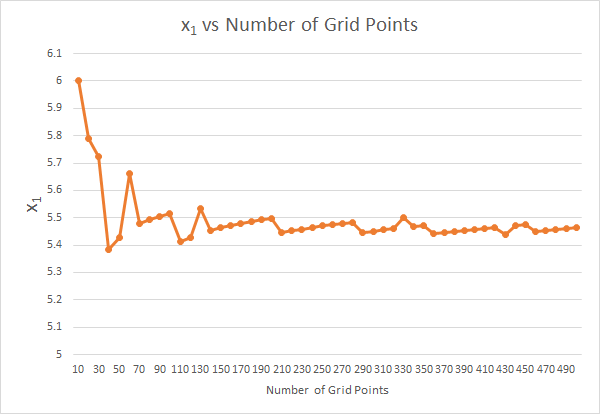
\includegraphics[width=10cm]{task5/task5-1.png} }}%
    \subfloat[$x_{2}$ as number of grid points increases]{{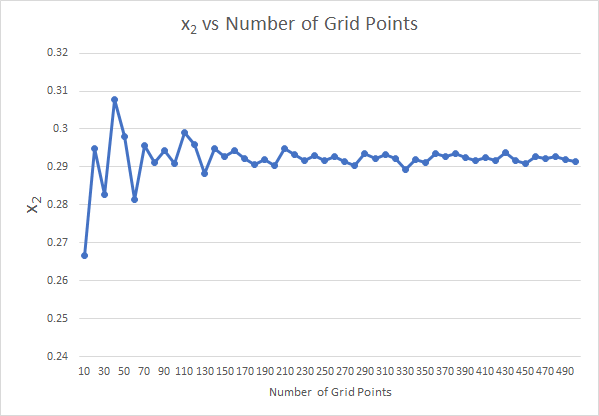
\includegraphics[width=10cm]{task5/task5-2.png} }}%
\end{adjustbox}
    \caption{$x_{1}$ and $x_{2}$ of found minimum as number of grid points increases}
    \label{fig:task5}%
\end{figure}
\FloatBarrier
\noindent It can be seen from Fig. \ref{fig:task5} above that with an increasing number of grid points, there is a corresponding increase in accuracy as $x_{1}$ and $x_{2}$ oscillate closer and closer to their true values. This is intuitive as with an increase in number of grid points, there are more points to search from within the same space of $2 \leq x_{1} \leq 14$, and $0.2 \leq x_{2} \leq 0.8$ as specified in the constraints of the design problem. This means that the chance that a grid point lay close to the true minimum solution increases with an increase in the number of grid points, which is an intuitive and expected result. The cost of this, is an increase in computation time to find the solution as there are more points to search through.
\end{document}
